%Matteo Kumar - Leonard Schatt
% Fortgeschrittenes Physikalisches Praktikum

\clearpage
\section{Fitten der Shockley-Gleichung}

Aus den Daten wurde mithilfe einens MatLab-Programmes ref die Parameter, welche in der Shockley-Gleichung vorkommen ref gefittet. Dabei wird beachtet, 
dass bei der CIS-Zelle einen Reihenschaltung von 11 kleinen Solarmodulen vorhanden ist. Daher wird die Spannung durch 11 geteilt. Leider erhält man 
trotzdem sehr fragwürdige Parameter, beispielsweise unrealistisch hohe Temperaturen als Umgebungsbedingungen hatten. Diese sind aber ausgeschlossen, 
da die Temperatur als Referenz gemessen wurde.
Interessant ist vorallem, dass sich mit dem Programm vor allem die Multi- und MonoSi besser mitder Shockley-Gleichung gefittet werden, als 
die CIS Solarzelle, was aber auch gut an der fehlerhaften Anwendung des Programmes oder dem Programm selbst.

\subsection{CIS-Solarmodul}

Nach dem fitten mit dem oben erwähnten Programm erhält man folgende Abbildungen und Parameter.

\begin{figure}[ht]
    \centering
    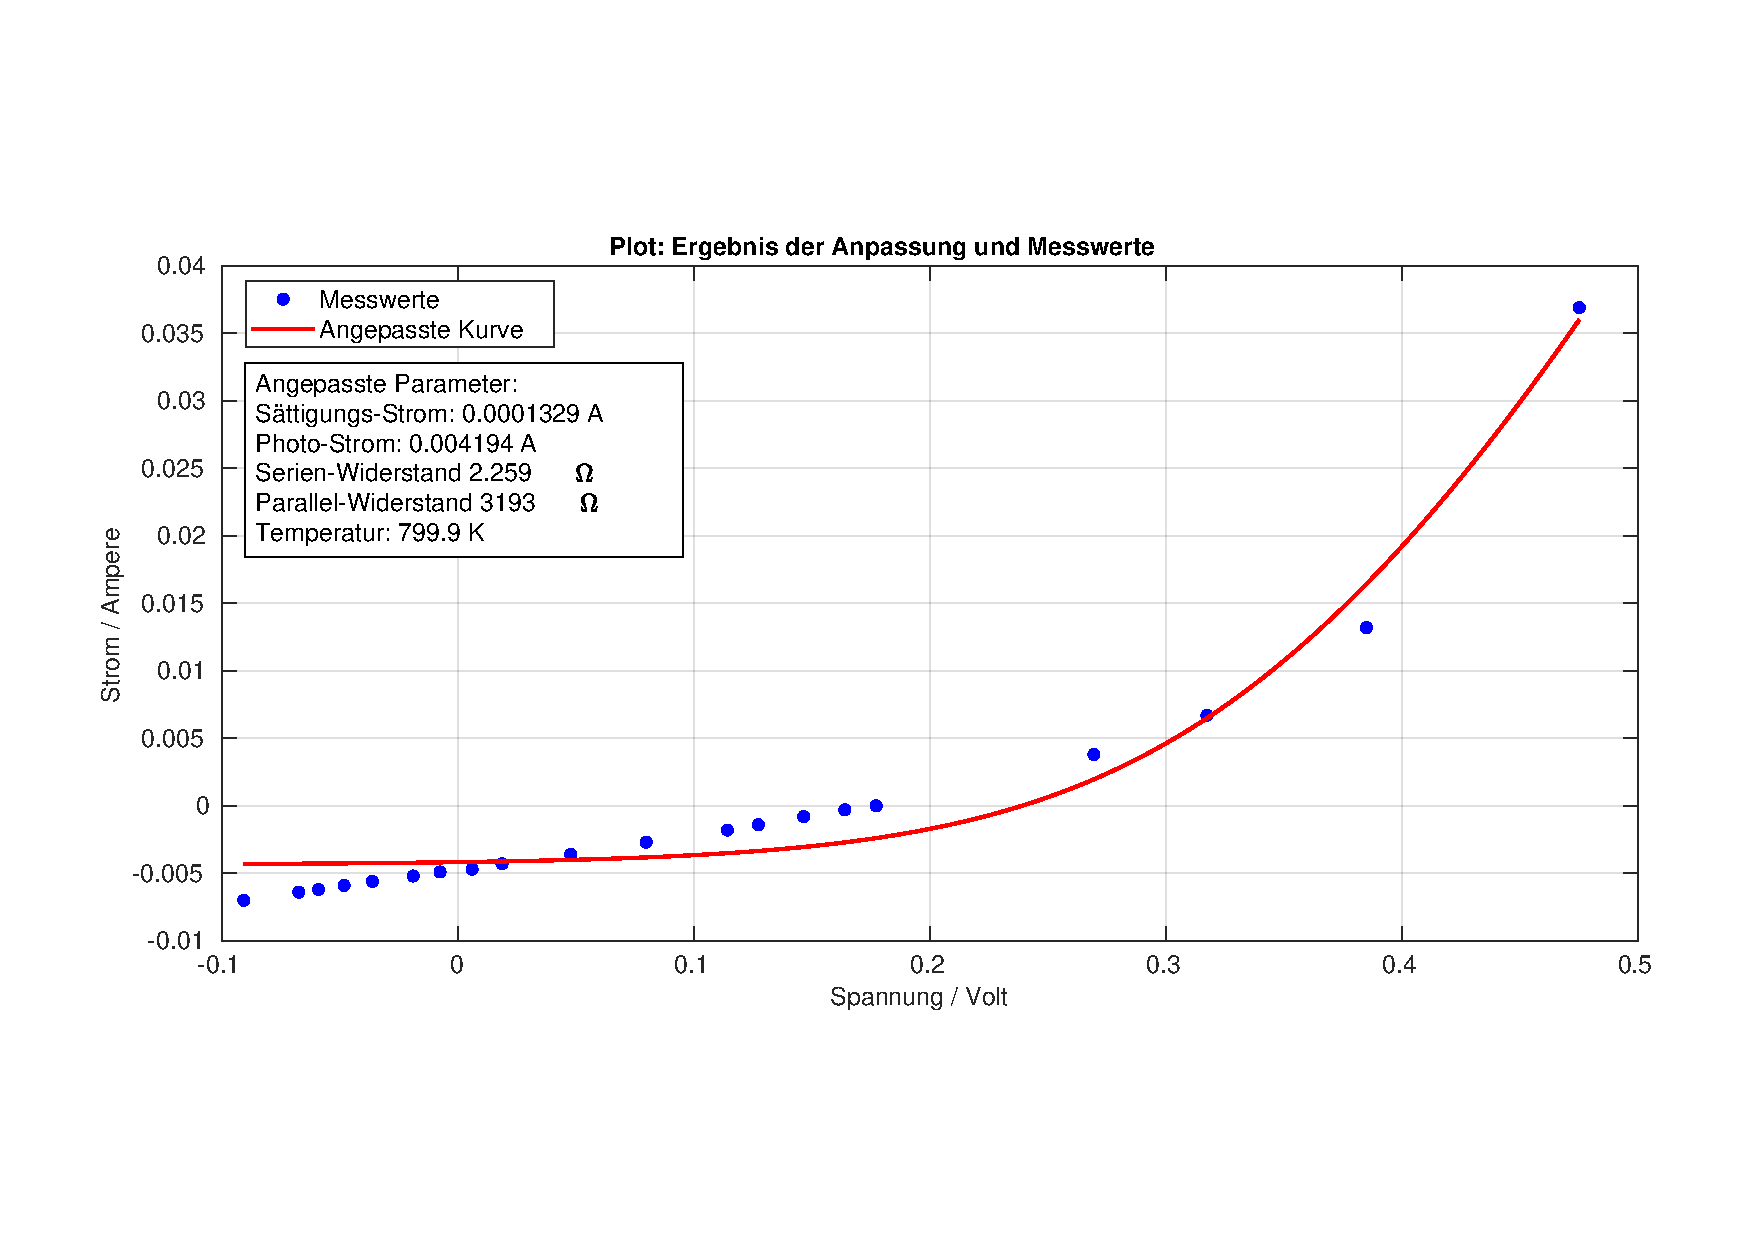
\includegraphics[width = \linewidth]{Bilder/CIS130Plot.pdf}
    \caption{Gefittete Shockley-Gleichung an das CIS-Modul bei 130V Trafospannung}
    
\end{figure}

\begin{figure}[ht]
    \centering
    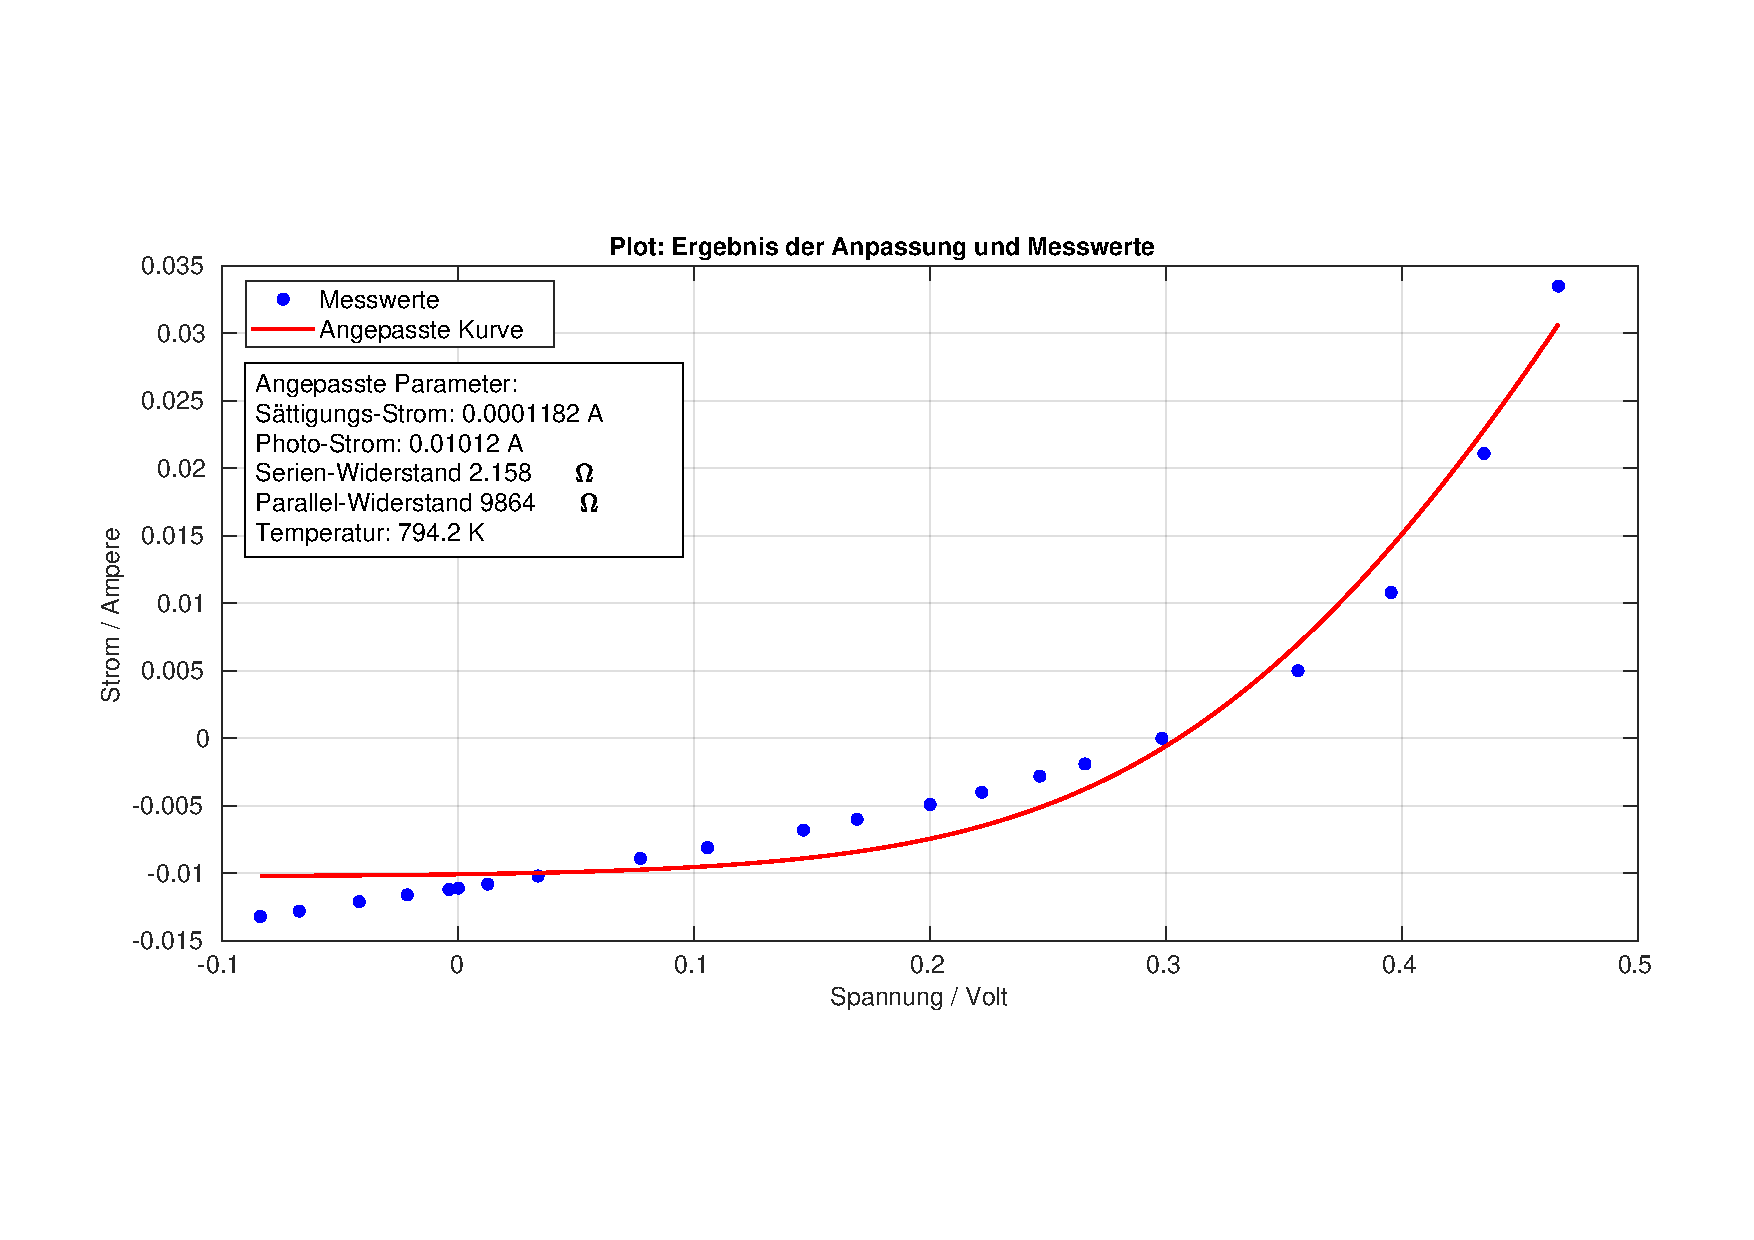
\includegraphics[width = \linewidth]{Bilder/CIS180Plot.pdf}
    \caption{Gefittete Shockley-Gleichung an das CIS-Modul bei 180V Trafospannung}    
\end{figure}

\begin{figure}[ht]
    \centering
    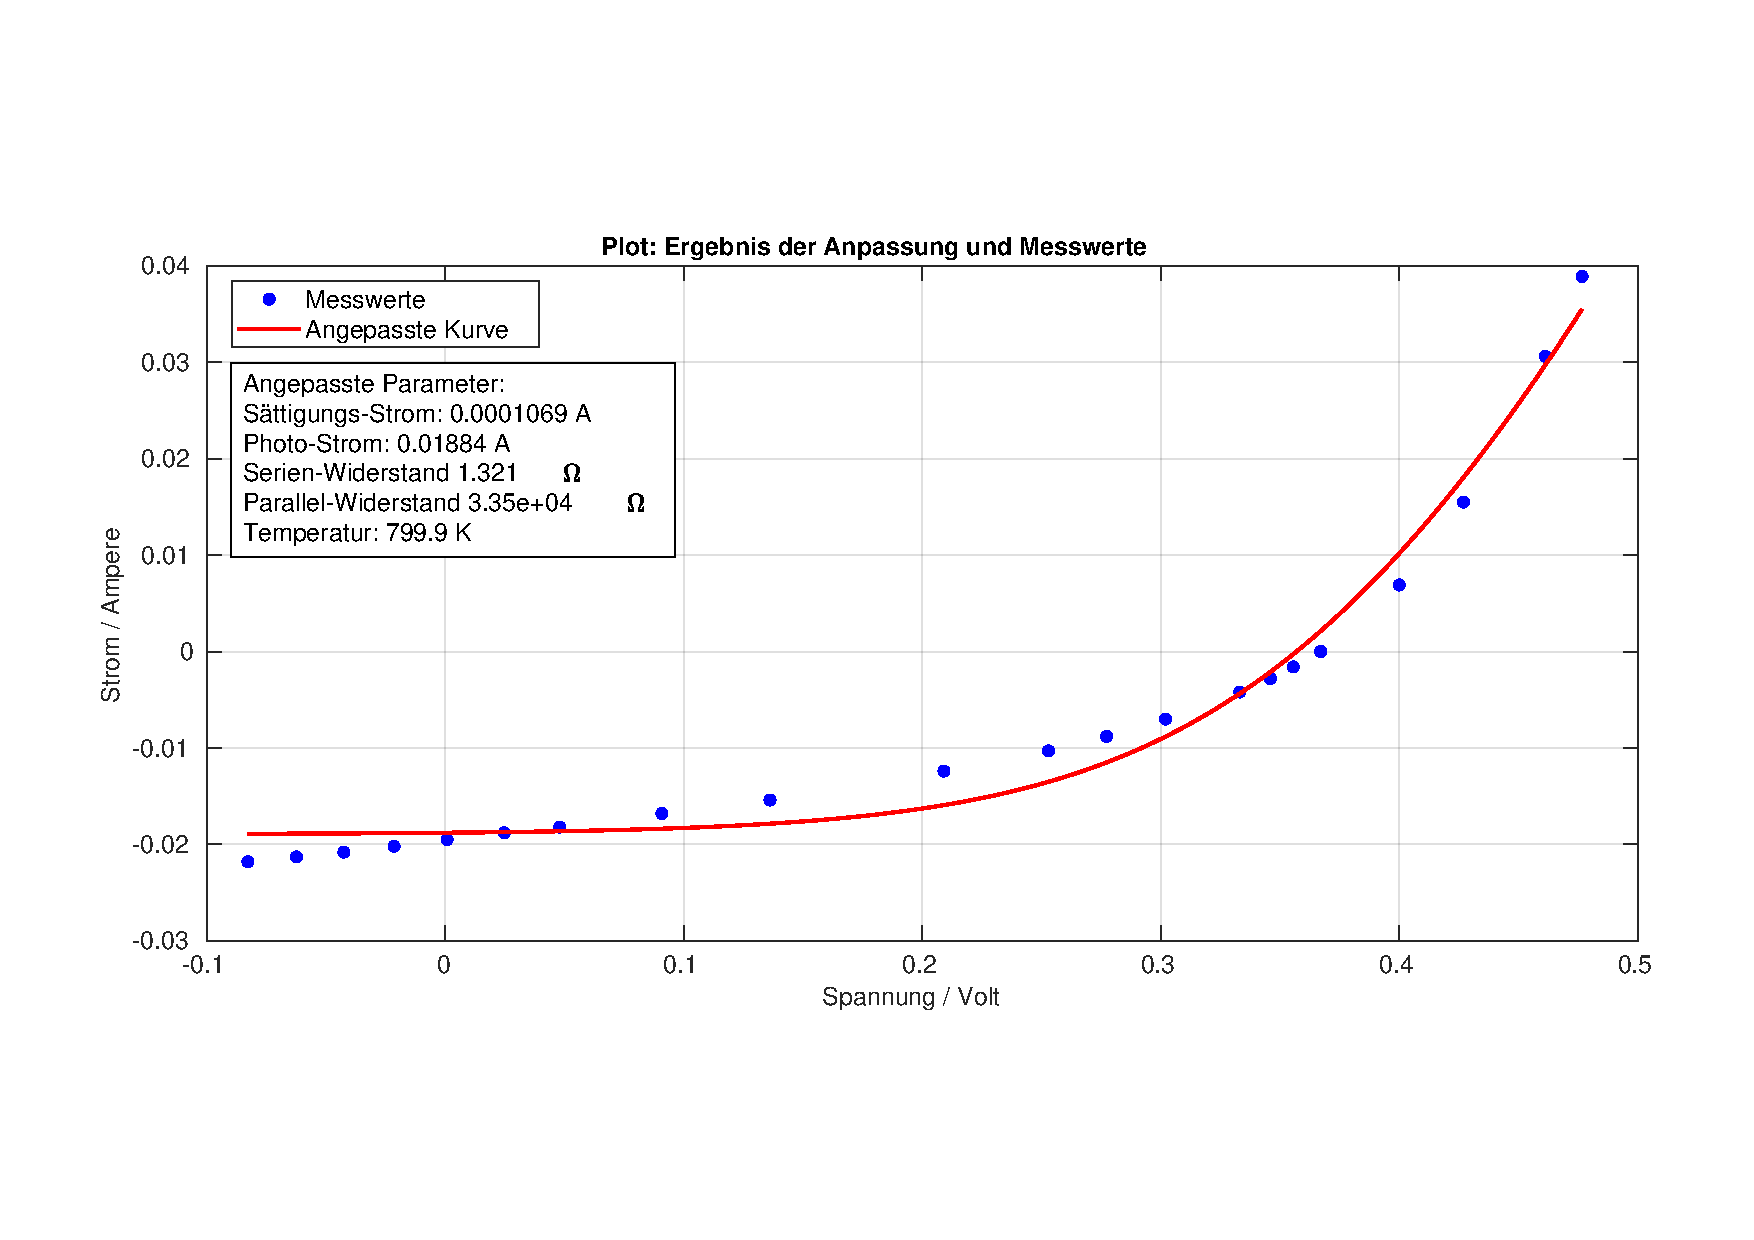
\includegraphics[width = \linewidth]{Bilder/CIS230Plot.pdf}
    \caption{Gefittete Shockley-Gleichung an das CIS-Modul bei 230V Trafospannung}
\end{figure}

Dabei fällt vor allem die ungewöhnlich hohe Temperatur, wie auch die riesigen Reihen- und Parallel-Widerstände auf. 
Da die Werte sehr unrealistisch erscheinen, ist darauf zu schließen, dass sich irgendwo ein Fehler eingschlichen hat, 
den wir leider auch bei genauer Betrachtung nicht ermitteln konnten.

\begin{figure}[ht]
    \centering
    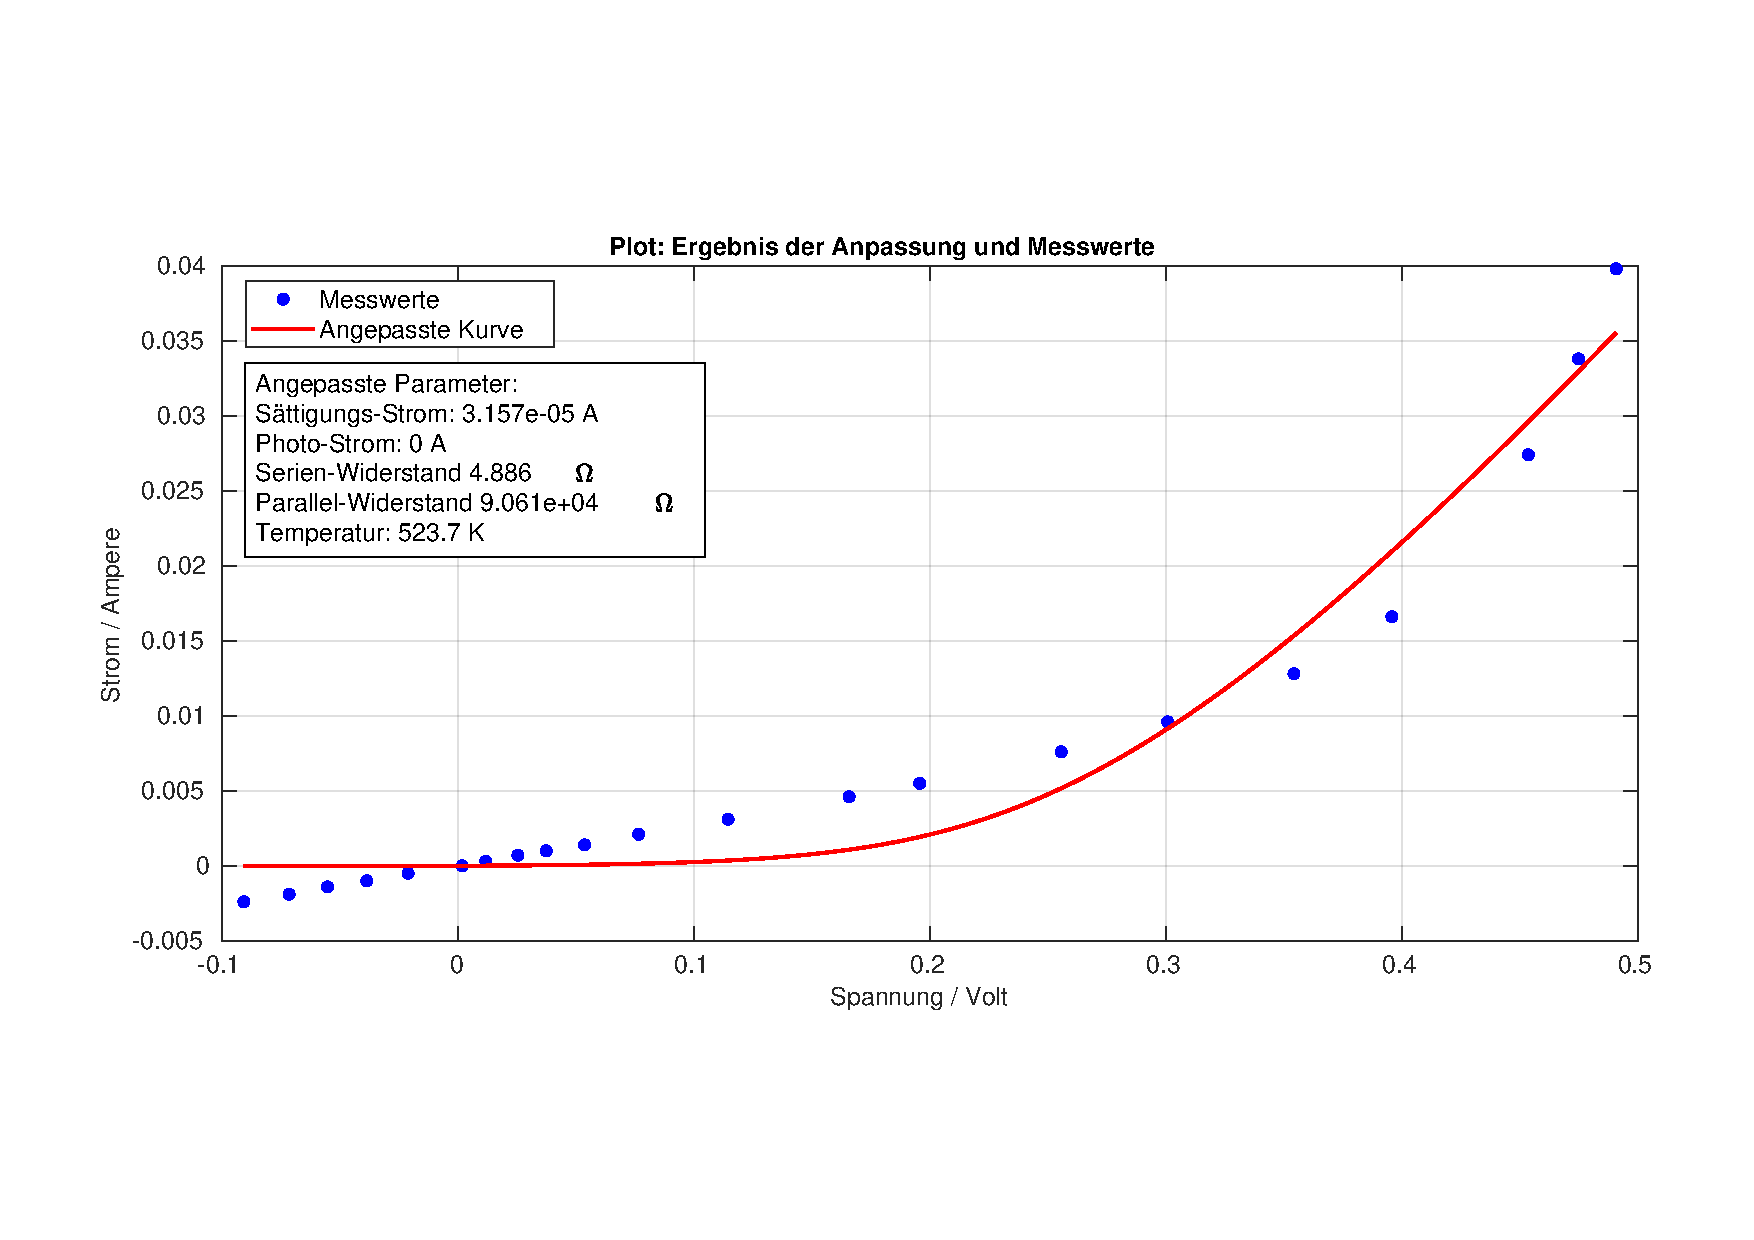
\includegraphics[width = \linewidth]{Bilder/CISDunkelPlot.pdf}
    \caption{Gefittete Schockley-Gleichung an Dunkelmessung der CIS-Zelle}
\end{figure}

\clearpage

\subsection{Mono- und MultiSi-Zellen}

Auch Mono- und MultiSi-Module wurden versucht mit dem Programm zu fitten. Dabei funktionierte das hier sichtlich besser.

\begin{figure}[ht]
    \centering
    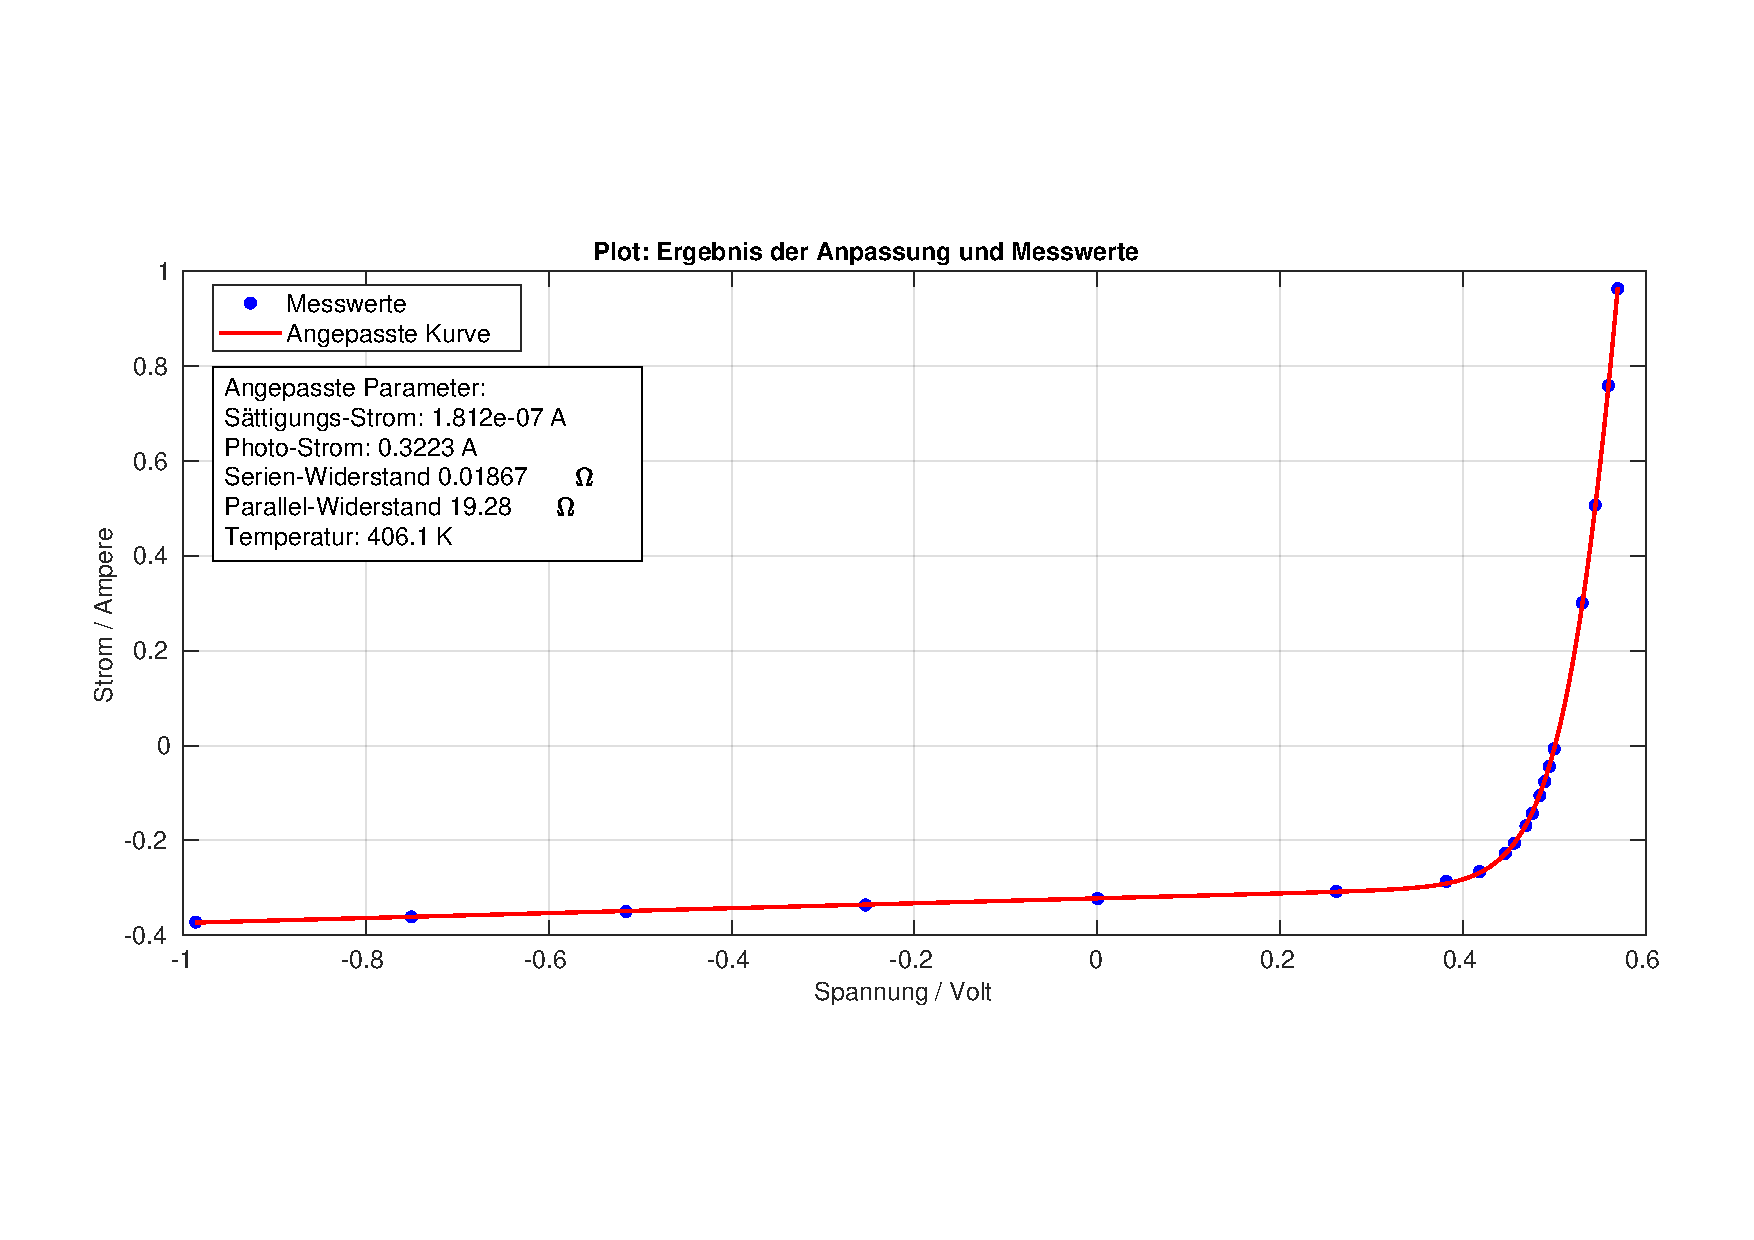
\includegraphics[width = \linewidth]{Bilder/SiMono130Plot.pdf}
    \caption{Gefittete Schockley-Gleichung an das Mono-Si-Modul bei 130V}
\end{figure}

\begin{figure}[ht]
    \centering
    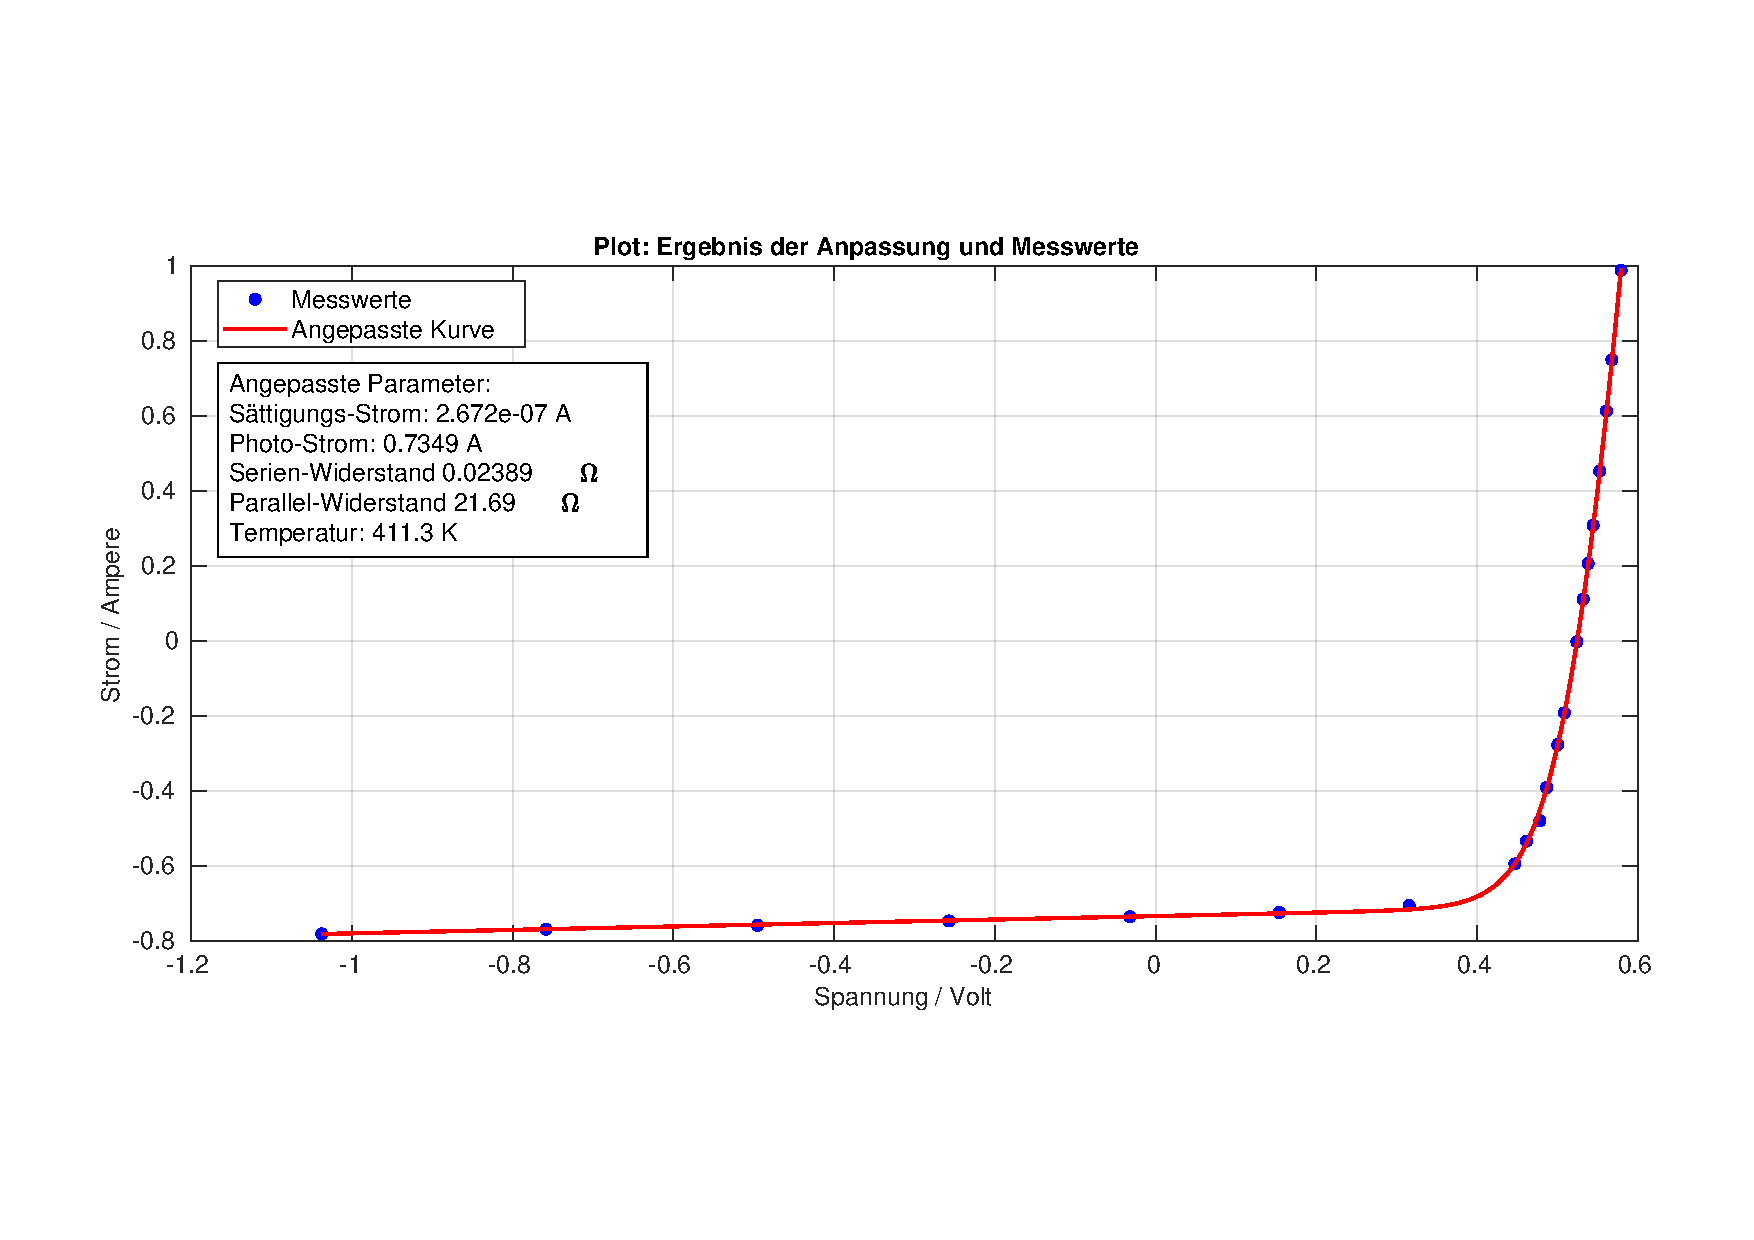
\includegraphics[width = \linewidth]{Bilder/SiMono180Plot.pdf}
    \caption{Gefittete Schockley-Gleichung an das Mono-Si-Modul bei 180V}
\end{figure}


\begin{figure}[ht]
    \centering
    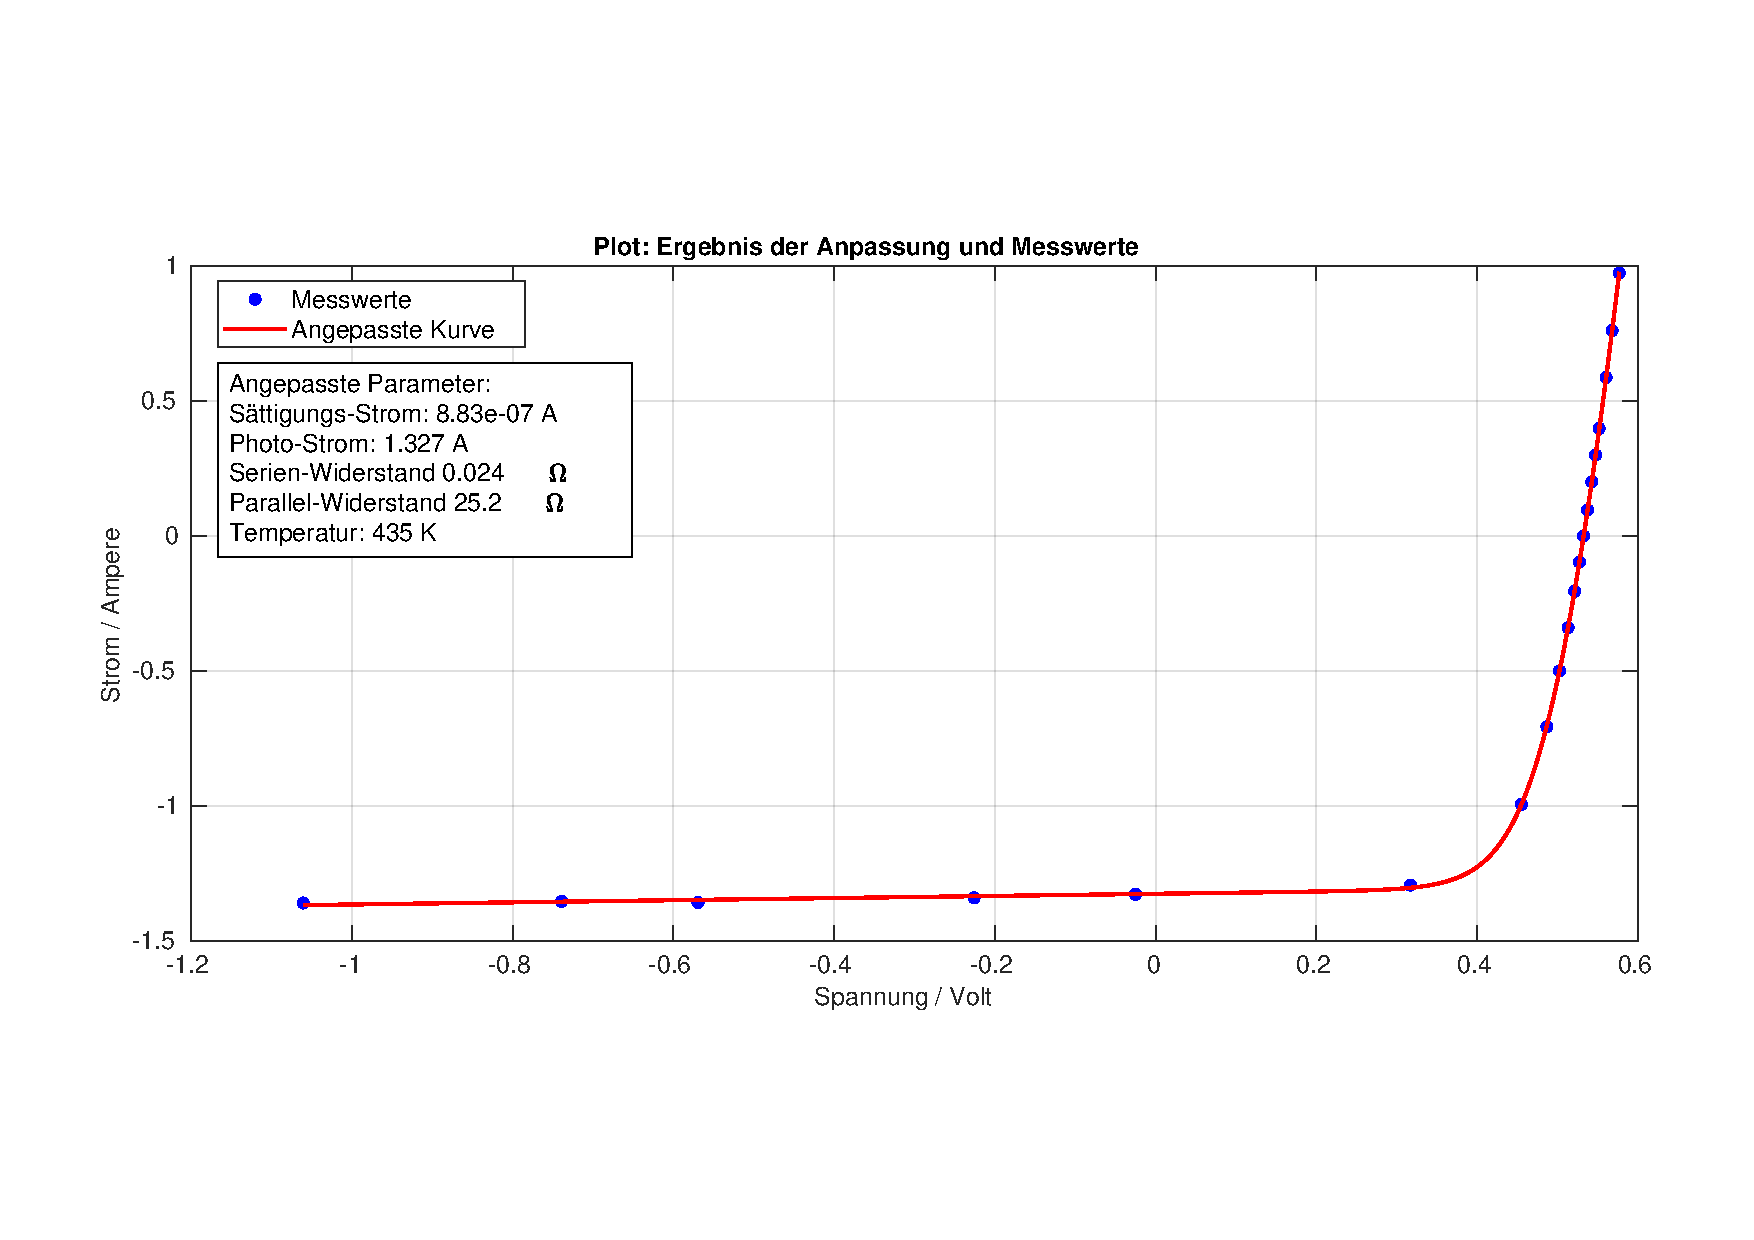
\includegraphics[width = \linewidth]{Bilder/SiMono230Plot.pdf}
    \caption{Gefittete Schockley-Gleichung an das Mono-Si-Modul bei 230V}
\end{figure}


Dabei ist, wie erwartet, der Photostrom $I_{Ph}$ bei steigender Helligkeit immer stärker. Die restlich Grafiken befinden sich im Anhang. Bei 
allen ist schön das "nach unten verschieben" bei höherer Lichtleistung beobachtbar. \\
Die Füllfaktoren $FF$ und Strom und Spannung am $MPP$ ergeben sich nach grafischer Auswertung wie folgt:\\
\begin{table}[h]
    \centering
    \begin{tabular}{l|c|c|r}
        & Strom am $MPP$ (A) & Spannung am $MPP$ (V) & $FF$ \\
        \toprule
        SiMono bei 130V & 0.405 & -0.27 & 0.69 \\
        SiMono bei 180V & 0.416 &-0.66 & 0.71 \\
        SiMono bei 230V & 0.412 & -1.19 & 0.69\\
        \midrule
        SiMulti bei 130V & 0.398 & -0.25 & 0.70 \\
        SiMulti bei 180V & 0.414 & -0.55 & 0.71 \\
        SiMulti bei 230V & 0.435 & -1.05 & 0.74\\
        \midrule
        CIS bei 130V & 0.151 &  -0.0029 & 0.44 \\
        CIS bei 180V & 0.202 & -0.0073 & 0.48 \\
        CIS bei 230V & 0.238 & -0.0144 & 0.51\\
    \end{tabular}
\end{table}

Dabei ist auffällig, dass am $MPP$ die Spannungswerte immer nahezu identisch sind. Die Stromwerte steigen aber eindeutig. Außerdem ist der 
niedrige Füllfaktor bei de, CIS-Modul auffällig. Daraus würde man ein langsames Ansteigen der Kurve vermuten, welches man dann im Bild auch beobachten kann. 
Die CIS-Zelle ist somit am weitesten von einer idealen Solarzelle entfernt, da sie den langsamen ansteig hat. Das erklärt auch, warum beim fitten die 
hohe Temperatur vorgeschlagen wird, da diese zu einem langsameren Anstieg der U_I_Kennlinie führt. Insgesamt beschreibt das Ersatzschaltbild 
die CIS-Zelle möglicherweise nicht gut.

\subsection{Idealitätsfaktor}